\documentclass[tikz,border=10pt]{standalone}
\usetikzlibrary{calc}
\begin{document}
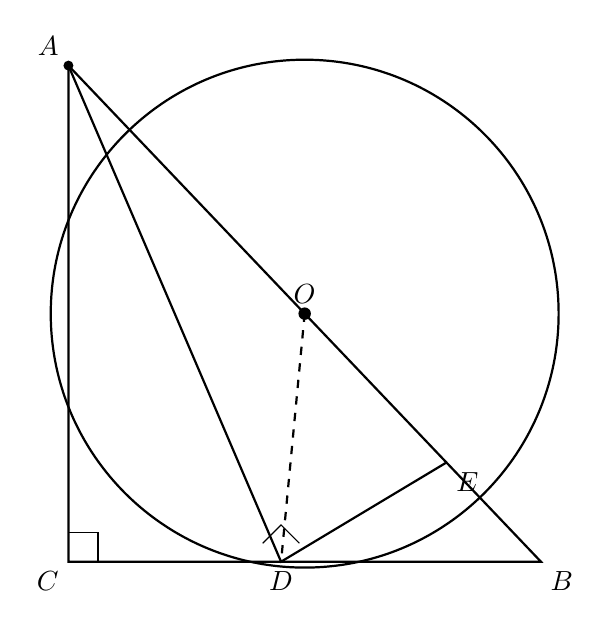
\begin{tikzpicture}[scale=1.5]
% Coordinates
\coordinate (C) at (0,0);
\coordinate (B) at (4,0);
\coordinate (A) at (0,4.2);
\coordinate (D) at (1.8,0);
\coordinate (O) at (2,2.1);
\coordinate (E) at ($(A)!0.8!(B)$);
% Circle through A, D, E centered at O
\draw[thick] (O) circle (2.15);
% Triangle ABC
\draw[thick] (A) -- (C) -- (B) -- cycle;
% Chords AD, DE
\draw[thick] (A) -- (D) -- (E);
% Dashed radius OD
\draw[dashed,thick] (O) -- (D);
% Right angle mark at C
\draw ($(C)+(0.25,0)$) -- ($(C)+(0.25,0.25)$) -- ($(C)+(0,0.25)$);
% Right angle mark at D (between OD and DE)
\draw[rotate around={45:(D)}] ($(D)+(0.22,0)$) -- ($(D)+(0.22,0.22)$) -- ($(D)+(0,0.22)$);
% Points
\fill (O) circle (1.5pt);
\fill (A) circle (1.2pt);
% Labels
\node[above left] at (A) {$A$};
\node[below left] at (C) {$C$};
\node[below] at (D) {$D$};
\node[below right] at (B) {$B$};
\node[above] at (O) {$O$};
\node[below right] at (E) {$E$};
\end{tikzpicture}
\end{document}
